	\subsubsection{Periodo di Avvio (2018-12-04 - 2018-12-17)}
		Nel periodo di avvio hanno luogo le seguenti attività:
		\begin{itemize}
			\item ricerca degli strumenti: tutti i membri del gruppo effettuano le ricerche sui possibili strumenti utili alle attività di avvio e di analisi dei requisiti;
			\item prima normazione: gli amministratori redigono le \textit{NormeDiProgetto\_v2.0.0} concordate per i processi di supporto e organizzativi;
			\item studio di fattibilità: gli analisti redigono lo \textit{StudioDiFattibilità\_v2.0.0} dei capitolati;
			\item pianificazione di progetto: il responsabile redige il \textit{PianoDiProgetto\_v2.0.0}, riportando modello di sviluppo, analisi dei rischi e la pianificazione per le prime attività dell'analisi dei requisiti;
			\item verifica dei documenti: i verificatori controllano che i documenti siano corretti.
		\end{itemize}
		
	\subsubsection{Periodo di Analisi dei Requisiti (2018-12-18 - 2019-01-21)}	
 Il periodo di analisi dei requisiti inizia con le attività di:
			\begin{itemize}
				\item pianificazione di progetto: il responsabile effettua il resoconto del periodo di avvio e pianifica in maniera più dettagliata le attività di analisi dei requisiti; 
				\item pianificazione della qualifica: i verificatori redigono il resoconto del periodo di avvio e gli amministratori effettuano i primi incrementi per il \textit{PianoDiQualifica\_v2.0.0};
				\item normazione: gli amministratori redigono in maniera precisa e completa le \textit{NormeDiProgetto\_v2.0.0} per l'attività di analisi;
				\item verifica dei documenti: si procede con la verifica del \textit{PianoDiProgetto\_v2.0.0}, del \textit{PianoDiQualifica\_v2.0.0} e delle \textit{NormeDiProgetto\_v2.0.0}.
				\item analisi dei requisiti del sistema: gli analisti svolgono la prima analisi dei requisiti del sistema;
				\item incrementi al \textit{PianoDiQualifica\_v2.0.0}: i verificatori introducono nel piano i test di sistema in base a quanto scaturito dall'analisi dei requisiti;
				\item verifica dell'analisi dei requisiti di sistema;
				\item incrementi all'analisi dei requisiti: gli analisti aggiungono degli incrementi all'analisi di sistema;
				\item verifica degli incrementi all'analisi dei requisiti;
				\item incrementi al \textit{PianoDiProgetto\_v2.0.0}: il responsabile redige la parte di rendicontazione e consuntivo del \textit{PianoDiProgetto\_v2.0.0} da presentare alla Revisione dei Requisiti.
				\item incrementi al \textit{PianoDiQualifica\_v2.0.0}: i verificatori redigono la parte di rendicontazione del \textit{PianoDiQualifica\_v2.0.0} da presentare alla Revisione dei Requisiti, aggiungendo i risultati delle misurazioni effettuate, e gli analisti aggiungono i restanti test di sistema;
				\item verifica del \textit{PianoDiProgetto\_v2.0.0} e del \textit{PianoDiQualifica\_v2.0.0};
				\item approvazione dei documenti da parte del responsabile;
				\item preparazione alla presentazione.			
			\end{itemize}
			
\begin{figure}[h]
	\centering
	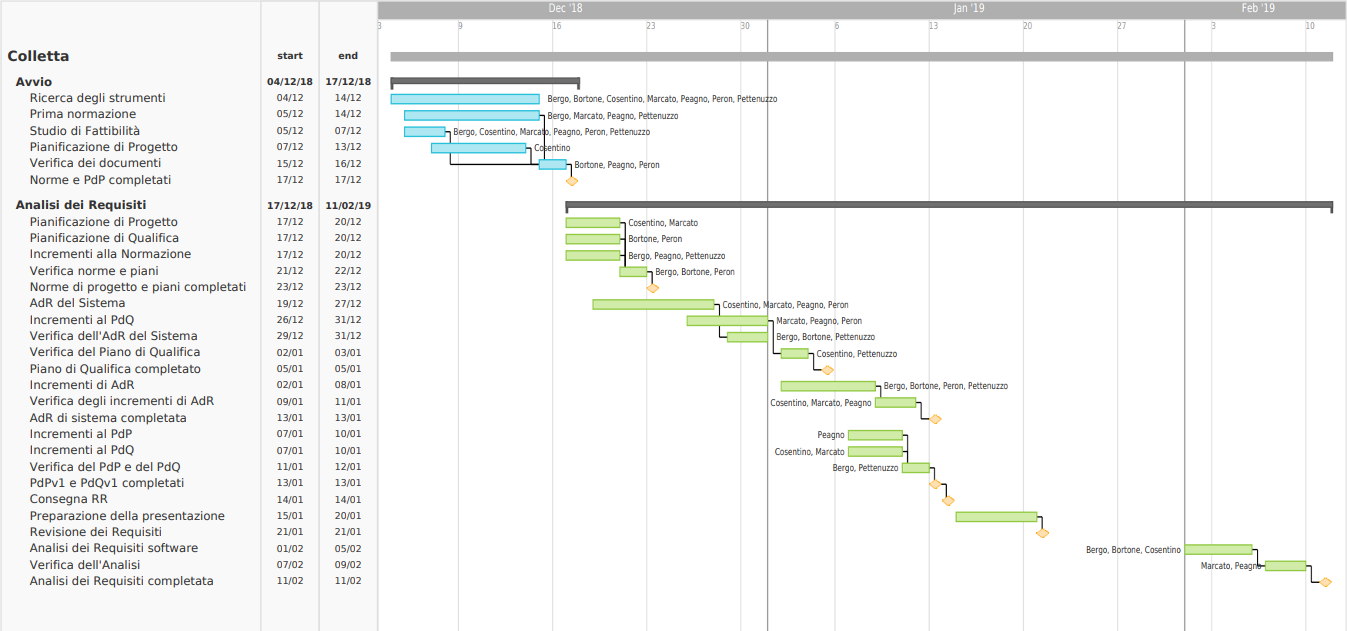
\includegraphics[scale=0.33]{images/ganttan.png}
	\caption{Diagramma di Gantt riguardante la fase 1}
\end{figure}